\chapter{Objetivos} 
%----------------------------------------------------------------------------------------
%	SECTION 1
%----------------------------------------------------------------------------------------
Una vez  hemos enfocado el contexto en el que se va a desarrollar este trabajo,pasamos a definir los objetivos que se pretenden cubrir en este TFG.

El objetivo principal es desarrollar un conjunto de practicas basadas en tecnologías web punteras para la asignatura de LTAW.Cada una se trata como un subobjetivo.

El primer subobjetivo es crear una aplicación Web enfocada en tecnologías del cliente.Por ello vamos a diseñar un juego en la web desatollado con HTML5 y JavaScript.

El segundo subobjetico es crear una aplicación web enfocada en tecnologías de comunicación bidireccional en tiempo real.En este caso se parte del primer subobjetivo ya que por medio de WebSockets se transforma en un juego online multijugador.

El tercer subobjetivo es crear una aplicación web enfocada en tecnologías de servidor con manejo de base de datos.Se desarrolla una Web de eventos y cantantes por medio de Django como framework utilizando la BBDD de MySQL.

El cuarto subobjetivo es crear una aplicación web enfocada en tecnologías de comunicación audiovisual.Se creara una sala de chat por medio de una conexion Peer-to-Peer entre navegadores desarrollado con WebRTC.

Como objetivo general de cada uno de las practicas es ser lo suficientemente maduras y aportar nuevas funcionalidades en el caso que se necesario para que de esta forma sirva como modelo a los alumnos de la asignatura de LTAW.
%----------------------------------------------------------------------------------------
%	SECTION 2
%----------------------------------------------------------------------------------------
\section{Metodología y plan de trabajo}
La realización de todo proyecto necesita una metodología a seguir con el que se planifica las tareas necesarias para llegar a nuestro objetivo. Por ello se ha seleccionado el modelo de desarrollo en espiral, figura \ref{fig:espiral},que se aplica habitualmente en ingeniería de software.
\\Este modelo define una serie de ciclos que se repiten continuamente hasta finalizar el proyecto, dividiéndolo en subtareas mas sencillas en las que se establece un punto de control al final de cada una para evaluar el resultado y establecer nuevas tareas.

Durante el tiempo que ha durado el proyecto se acordaron reuniones semanales con el tutor de forma presenciales o por Video-Conferencia en las que se revisaba los objetivos semanas y se definían los nuevos objetivos.
\\Los avances mas relevantes se añadían a la mediawiki \cite{Mediawiki} de JdeRobot y a través de repositorio de GitHub \cite{Repositorio} guardábamos el código.
\\Para finalizar este capitulo explicamos las distintas partes en las que se ha divido el plan del proyecto.
\begin{enumerate}
\item \textbf{Aprendizaje de tecnologías web:} Estudiar y conocer distintas tecnologías web del servido, cliente, BBDD y tecnologías de intercambio de información entre el cliente y el servidor.
\item \textbf{Selección de practicas:} Con los conocimientos adquiridos realizamos una propuesta que se ajuste a los requisitos marcados.
\item \textbf{Desarrollo de practicas:} El diseño y desarrollo de cada practica ha sido de forma incremental,es decir,se ha buscado obtener la funcionalidad exigida en cada una para luego centrarnos en dar una apariencia mas atractiva.
\item \textbf{Experimentos:} Cada una de las practicas serán probadas por una terceras personas para validar que la funcionalidad sea correcta.
\end{enumerate}
\begin{figure}[!h]
\centering
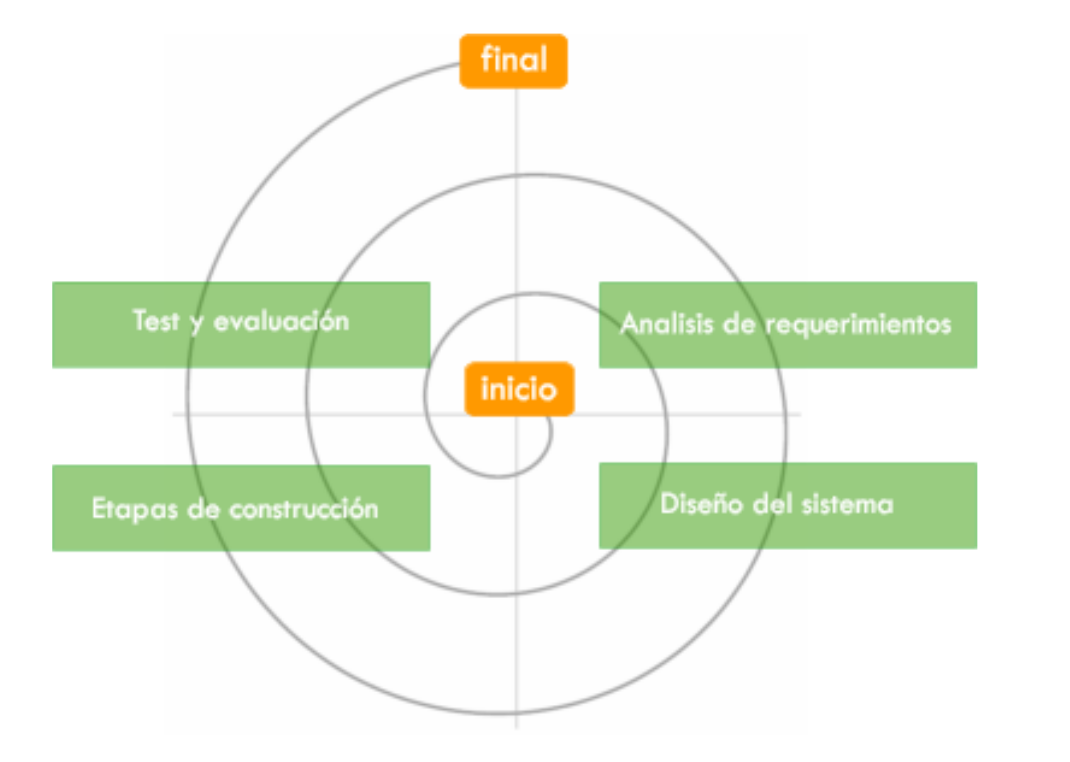
\includegraphics[width=0.8\linewidth]{Figures/espiral}
\decoRule
\caption[Metodología en espiral]{Metodología en espiral.}
\label{fig:espiral}
\end{figure}
